\documentclass[12pt]{article}
\usepackage{ctex}
\usepackage{graphicx}
\usepackage{indentfirst}
\usepackage{amsmath}
\usepackage{float}
\usepackage{amssymb}

\title{第五周作业报告}
\author{佐藤拓未 20300186002}
\date{}

\begin{document}
	\maketitle
	\begin{center}
		\textbf{第一问}
	\end{center}
用二阶到四阶格式计算例2.2.2, 观察收敛阶\\
\\
\textbf{解:}考虑用MATLAB计算例2.2.2, 先设$t_0=0, u_0=u(t_0)=2, T=1, \Delta{t}=2^{-i}, N= [\frac{T}{\Delta{t}}] $, 令$ i$变动, 这样可以后续观察收敛阶与$i$之间的关系. 又可知精确解$u(t)=\frac{1}{1-0.5e^{-t}}$, 编写子程序并带入参数计算, 给出二到四阶Kutta格式与精确解的末项相对误差与$i$之间的关系(如图1所示).\\
那么此时$u_N$就是在$T=1$处的近似值, 且$$\vert e_N \vert=\frac{\vert u(T)-u_N\vert}{\vert u(T)\vert}=O(\Delta{t}^p)\overset{\triangle}{=}C\Delta{t}^p$$
\noindent 则在对数意义下, 相对误差的对数值与$i$就呈现线性关系 $$\ln \vert e_N\vert = \ln C + p \ln{\Delta{t}} $$
\noindent 再由$\Delta{t}=\frac{1}{2^i}$, 可知 $$\ln \vert e_N\vert = \ln C - pi\ln2$$
\noindent 即斜率就是$-p\ln2$, 从而可以从图1的斜率差别观察到Kutta二至四阶的收敛阶.


\begin{figure}[H]
	\centering
	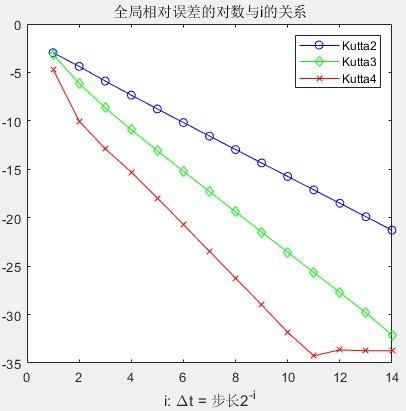
\includegraphics[width=0.85\textwidth]{1}
	\caption{相对误差的对数与$i$的关系}
\end{figure}
\noindent 而当$\Delta{t}\le 2^{-11}$时, Kutta四阶格式已经达到了机器精度, 从而收敛精度不会再进一步降低.\\
另一方面, 可以直接在数值上对比相对误差对数与$i$关系图以及斜率为$-p\ln2$的直线之间的关系, 如图2或者semilogy图(图3)所示.
\begin{figure}[H]
	\centering
	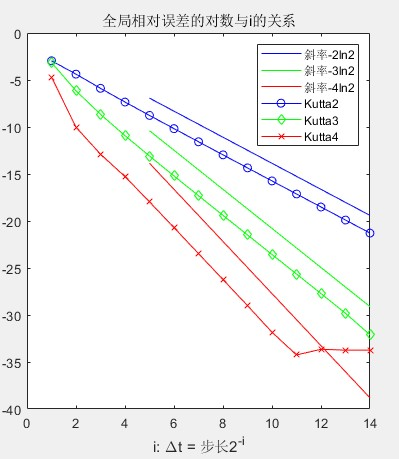
\includegraphics[width=0.85\textwidth]{2}
	\caption{图1的基础上加入直线作比较}
\end{figure}
\begin{figure}[H]
	\centering
	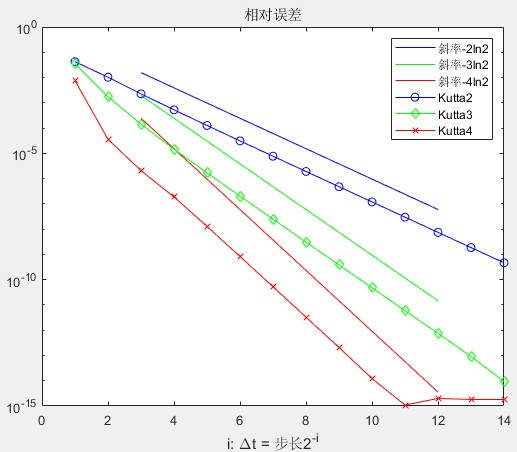
\includegraphics[width=0.85\textwidth]{3}
	\caption{semilogy}
\end{figure}
\noindent 从上图也可以看出Kutta的$p$阶格式与斜率为$-p\ln2$的直线之间的关系: 下降速度是接近的.\\


\begin{center}
	\textbf{第二问}
\end{center}
如果增量函数$\phi(t,u;\Delta{t})$在区域定义域上连续且关于$u$满足Lipschitz条件, 则相容得单步方法时收敛的, 且如果有局部截断误差:$$\vert R_n\vert\le C_R{\Delta{t}}^{p+1},$$
\noindent 则有收敛性估计$$\vert \epsilon_n \vert\le e^{L(T-t_0)} \vert e_0 \vert+{\Delta{t}}^{p}\frac{C_R}{L}e^{L(T-t_0)}$$
\\
\textbf{证:}考虑单步方法与局部截断误差
\begin{align*}
	\begin{cases}
		u_n &= u_{n-1} + \Delta{t}\phi(t_{n-1},u_{n-1};\Delta{t})\\
		u(t_n) &= u(t_{n-1}) + \Delta{t}\phi(t_{n-1},u(t_{n-1});\Delta{t})+R_n
	\end{cases}
\end{align*}
\noindent 由$\epsilon_n=u_(t_n)-u_n$, 以及$\phi(t,u;\Delta{t})$是关于$u$为$L$-Lipschitz连续, 可知
\begin{align*}
	\vert \epsilon_n\vert &\le \vert \epsilon_{n-1} \vert + L\Delta{t}\vert \epsilon_{n-1} \vert + \vert R_n\vert \\
	&=(1+L\Delta{t})\vert \epsilon_{n-1}\vert + C_R {\Delta{t}}^{p+1}\\
	&\le (1+L\Delta{t})^n\vert \epsilon_0\vert + C_R {\Delta{t}}^{p+1}\frac{1-(1+L\Delta{t})^n}{1-(1+L\Delta{t})}
\end{align*}
\noindent 由$(1+L\Delta{t})^n \le e^{nL\Delta{t}}$, 以及$T-t_0 \ge t_n-t_0=n\Delta{t}$, 可知
\begin{align*}
	\vert \epsilon_n\vert &\le e^{nL\Delta{t}}\vert \epsilon_0\vert + {\Delta{t}}^{p+1}C_R\frac{e^{nL\Delta{t}}}{L\Delta{t}}\\
	&\le e^{n(T-t_0)}\vert \epsilon_0\vert +{\Delta{t}}^p \frac{C_R}{L}e^{n(T-t_0)}
\end{align*}

	
	
	
	
\end{document}